\section{Resultados}

\subsection{\label{sub:data}Datos}

Tabla de alargamiento

%Tabla
\begin{table}[tbh]
    \caption{\label{tab:y}Muelle 1 - Alargamiento.}
    \begin{centering}
        \begin{tabular}{|P{37px}|P{53px}|P{37px}|P{53px}|}
            \hline
            $m$(g)    & $m + m_0$(g) & $y$(mm)    & $y - y_0$ (mm)                        \\
            \hline
            \csvreader[late after line= \\]{./files/data/1-y.csv}{}% use head of csv as column names
            {\csvcoli & \csvcolii    & \csvcoliii & \csvcoliv}% specify your columns here
            \hline
        \end{tabular}
    \end{centering}
\end{table}

Tabla de toma de tiempos


\begin{table}[tbh]
    \caption{\label{tab:t1}Muelle 1 - Tiempo.}
    \begin{centering}
        \begin{tabular}{|P{25px}|P{25px}P{25px}P{25px}|P{28px}P{28px}|}
            \hline
            $m$(g)    & $t_1$(s)  & $t_2$(s)   & $t_3$(s)  & $\langle t \rangle$(s) & $s$(s)                                \\
            \hline
            \csvreader[late after line= \\]{./files/data/1-t1.csv}{}% use head of csv as column names
            {\csvcoli & \csvcolii & \csvcoliii & \csvcoliv & \csvcolv               & \csvcolvi}% specify your columns here
            \hline
        \end{tabular}
    \end{centering}
\end{table}

Tabla de c�lculo del periodo

\begin{table}[tbh]
    \caption{\label{tab:t2}Muelle 1 - Periodo.}
    \begin{centering}
        \begin{tabular}{|P{40px}|P{40px}|P{50px}|P{50px}|}
            \hline
            $m$(g)    & $t$(s)    & $T = t / n$(s) & $T^2$(s)                              \\
            \hline
            \csvreader[late after line= \\]{./files/data/1-t2.csv}{}% use head of csv as column names
            {\csvcoli & \csvcolii & \csvcoliii     & \csvcoliv}% specify your columns here
            \hline
        \end{tabular}
    \end{centering}
\end{table}

asdfasdf

%Figura
\begin{figure}[tbh]
    \begin{centering}
        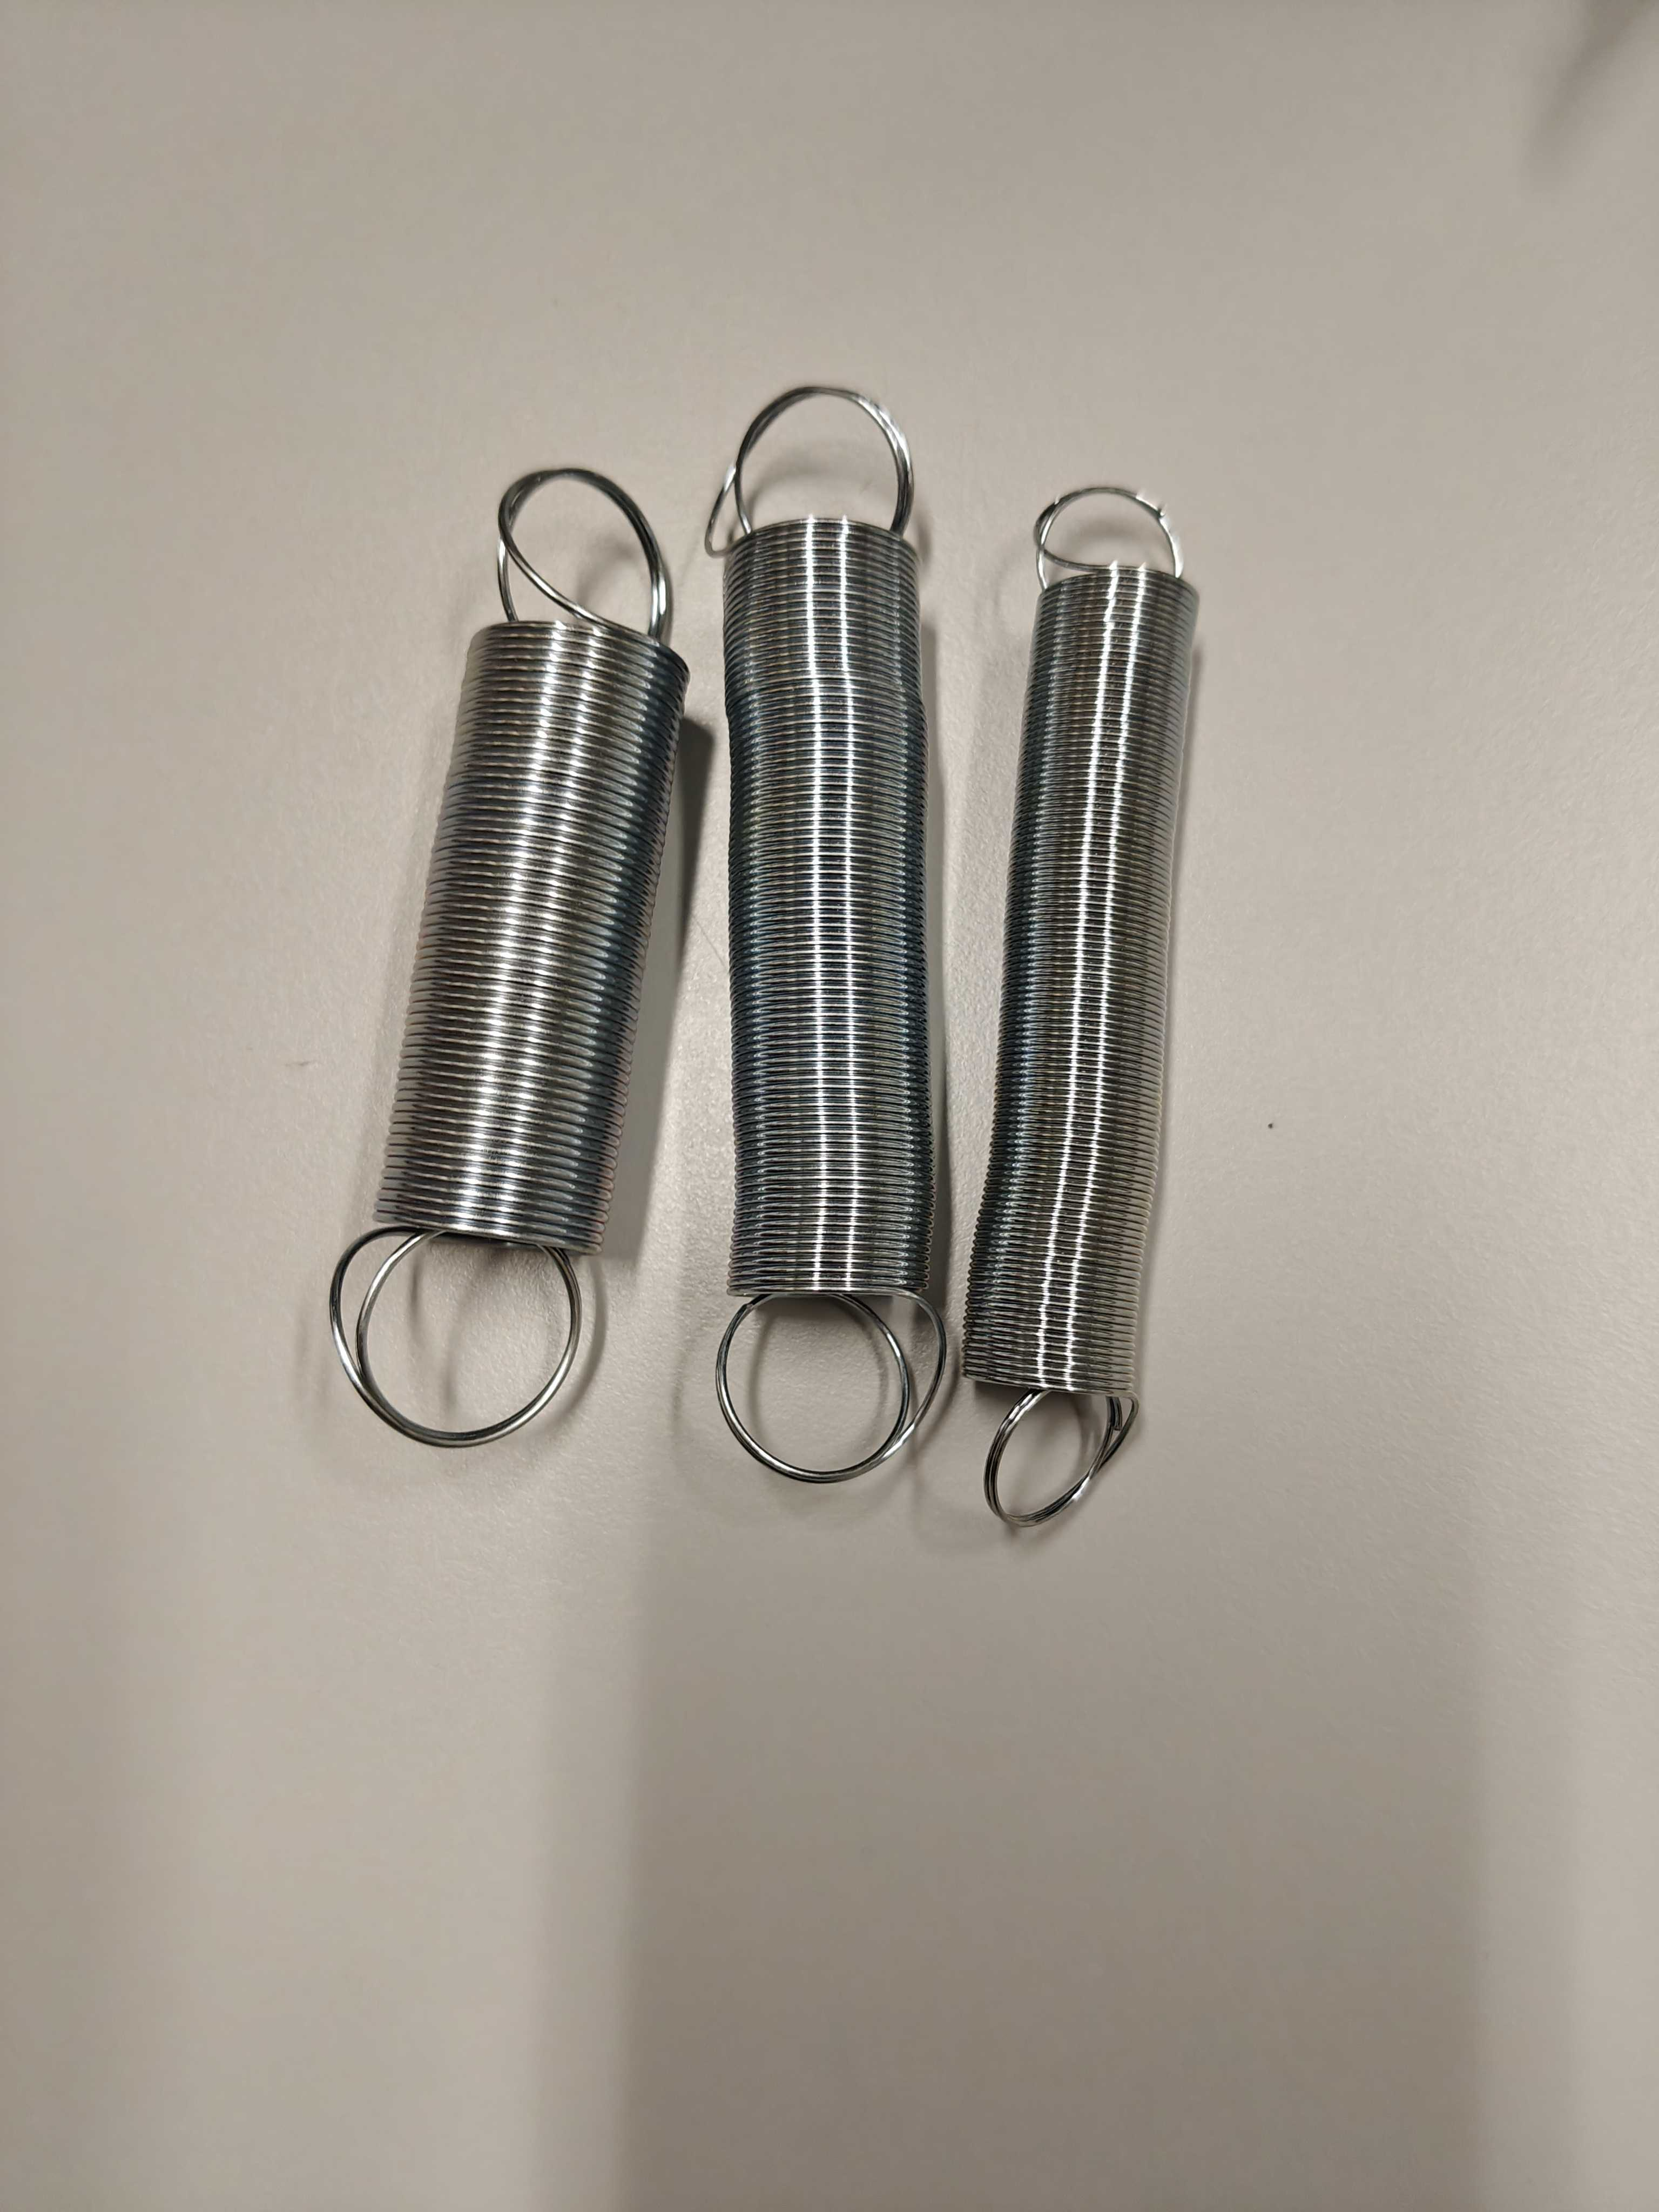
\includegraphics[width=0.8\columnwidth]{files/images/muelles}
    \end{centering}
    \caption{\label{fig:resultado}Miniatura de la primera p�gina de la plantilla
    de memoria.}
\end{figure}

\subsection{\label{sub:results}An�lisis}

Represente la deformaci�n frente a

